% $Id: results.tex 1784 2012-04-27 23:29:31Z nicolas.cardozo $
% !TEX root = main.tex

\chapter{Analysis and Results}
\label{cha:results}
As said before the anonymized results are found at \href{https://uniandes-my.sharepoint.com/:x:/g/personal/la_rodriguez_uniandes_edu_co/ESDy89Q-PgVBpYHEZ_CDh_IBhjhS35VFqNrlEjVw_ShY1w?e=lm319K}{this link}.
In this section the results of the survey presented in \fref{sec:evaluation} are presented and analyzed. This section 
is divided by the three main sections of the survey: \fref{sec:general-knowledge}, \fref{sec:tasks-results} and 
\fref{sec:usability}. Additionally, a discussion \fref{sec:discussion} section is added in which we analyze the results 
from the survey.

\section{General Knowledge Results}
\label{sec:general-knowledge}
Most of the people that answer the survey were very experienced on the use of python, as they used it very often in 
their work spaces and for the university tasks. Also, most of the people were very familiarized using \ac{RL} algorithms,
as they were taking the course. Nevertheless, the avarage of the students weren't familiarized with 
debuggers, they only used one very rarely, or used Visual Studio code interface for debugging.

\begin{figure}[!h]
    \centering
    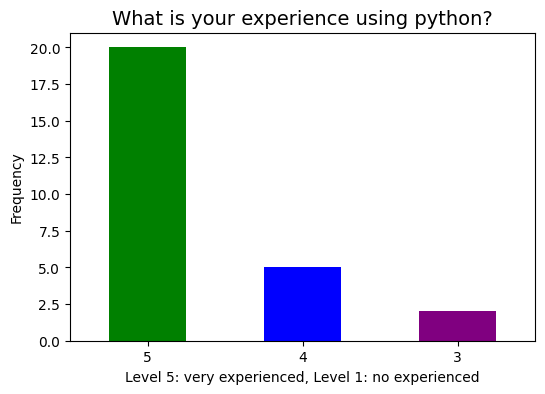
\includegraphics[width=0.5\textwidth]{figures/experience-python.png}
    \caption{Experience with Python}
    \label{fig:exp-py}
\end{figure}

\begin{figure}[!h]
    \centering
    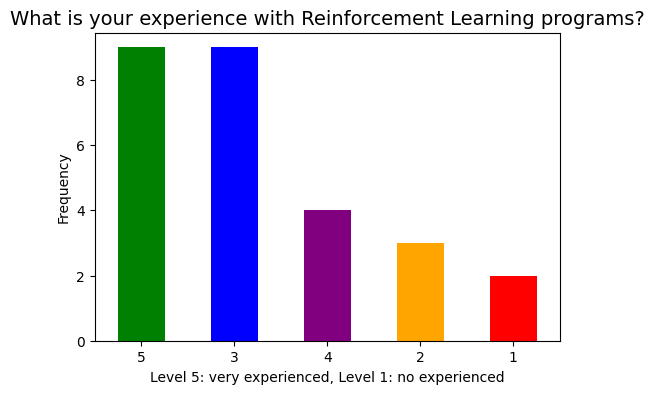
\includegraphics[width=0.5\textwidth]{figures/experience-rl.png}
    \caption{Experience with RL}
    \label{fig:exp-rl}
\end{figure}

\begin{figure}[!h]
    \centering
    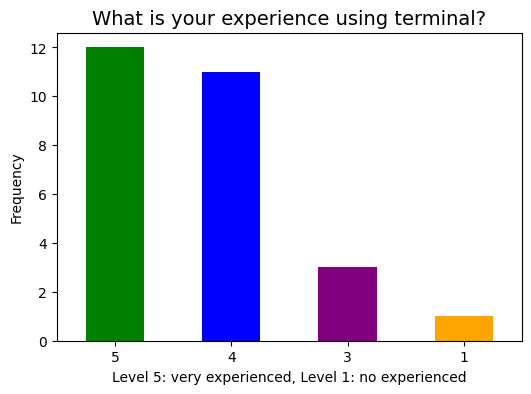
\includegraphics[width=0.5\textwidth]{figures/experience-terminal.png}
    \caption{Experience with Terminal}
    \label{fig:exp-terminal}
\end{figure}

\begin{figure}[!h]
    \centering
    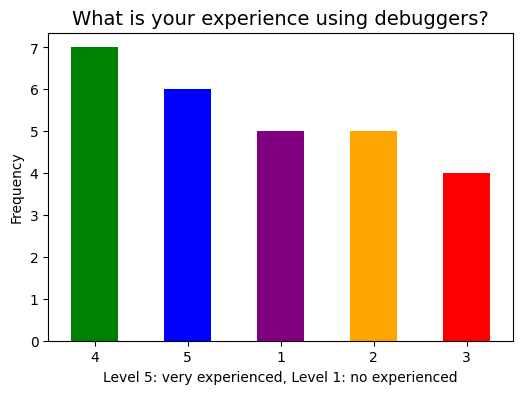
\includegraphics[width=0.5\textwidth]{figures/experience-debuggers.png}
    \caption{Experience with Debuggers}
    \label{fig:exp-deb}
\end{figure}

\section{Tasks Results}
\label{sec:tasks-results}

gridworld
\begin{table}[!h]
\centering
\resizebox{\columnwidth}{!}{%
\begin{tabular}{cccc}
\multicolumn{4}{c}{{\color[HTML]{000000} \textbf{Task 1: Gridworld Experiment.}}}                                                                                                                                                              \\
{\color[HTML]{000000} \textbf{Values}} & {\color[HTML]{000000} \textbf{Did you manage to finish the task?}} & {\color[HTML]{000000} \textbf{It was easy to solve the task}} & {\color[HTML]{000000} \textbf{Time it took you to find the bug}} \\
{\color[HTML]{000000} \textbf{5}}      & {\color[HTML]{000000} 15.0}                                        & {\color[HTML]{000000} 2}                                      & {\color[HTML]{000000} 2}                                         \\
{\color[HTML]{000000} \textbf{4}}      & {\color[HTML]{000000} 10.0}                                        & {\color[HTML]{000000} 16}                                     & {\color[HTML]{000000} 12}                                        \\
{\color[HTML]{000000} \textbf{3}}      & {\color[HTML]{000000} 2.0}                                         & {\color[HTML]{000000} 5}                                      & {\color[HTML]{000000} 4}                                         \\
{\color[HTML]{000000} \textbf{2}}      & {\color[HTML]{000000} NaN}                                         & {\color[HTML]{000000} 3}                                      & {\color[HTML]{000000} 8}                                         \\
{\color[HTML]{000000} \textbf{1}}      & {\color[HTML]{000000} NaN}                                         & {\color[HTML]{000000} 1}                                      & {\color[HTML]{000000} 1}                                        
\end{tabular}%
}
\end{table}

\begin{figure}[h]
    \centering
    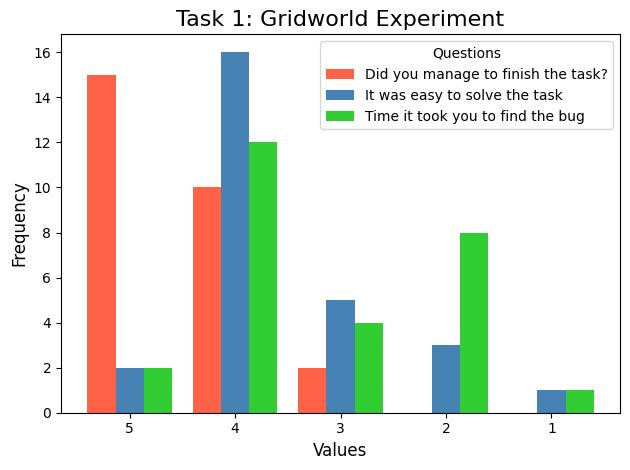
\includegraphics[width=0.5\textwidth]{figures/task1.png}
    \caption{Results Task 1}
    \label{fig:task1}
\end{figure}


rooms
\begin{table}[!h]
\centering
\resizebox{\columnwidth}{!}{%
\begin{tabular}{
>{\columncolor[HTML]{FFFFFF}}c 
>{\columncolor[HTML]{FFFFFF}}c 
>{\columncolor[HTML]{FFFFFF}}c 
>{\columncolor[HTML]{FFFFFF}}c }
\multicolumn{4}{c}{\cellcolor[HTML]{FFFFFF}{\color[HTML]{000000} \textbf{Task 2: Rooms Experiment.}}}                                                                                                                                          \\
{\color[HTML]{000000} \textbf{Values}} & {\color[HTML]{000000} \textbf{Did you manage to finish the task?}} & {\color[HTML]{000000} \textbf{It was easy to solve the task}} & {\color[HTML]{000000} \textbf{Time it took you to find the bug}} \\
{\color[HTML]{000000} \textbf{4}}      & {\color[HTML]{000000} 13}                                          & {\color[HTML]{000000} 8}                                      & {\color[HTML]{000000} 5}                                         \\
{\color[HTML]{000000} \textbf{5}}      & {\color[HTML]{000000} 7}                                           & {\color[HTML]{000000} 1}                                      & {\color[HTML]{000000} 4}                                         \\
{\color[HTML]{000000} \textbf{3}}      & {\color[HTML]{000000} 4}                                           & {\color[HTML]{000000} 11}                                     & {\color[HTML]{000000} 9}                                         \\
{\color[HTML]{000000} \textbf{1}}      & {\color[HTML]{000000} 2}                                           & {\color[HTML]{000000} 1}                                      & {\color[HTML]{000000} 3}                                         \\
{\color[HTML]{000000} \textbf{2}}      & {\color[HTML]{000000} 1}                                           & {\color[HTML]{000000} 6}                                      & {\color[HTML]{000000} 6}                                        
\end{tabular}%
}
\end{table}

\begin{figure}[h]
    \centering
    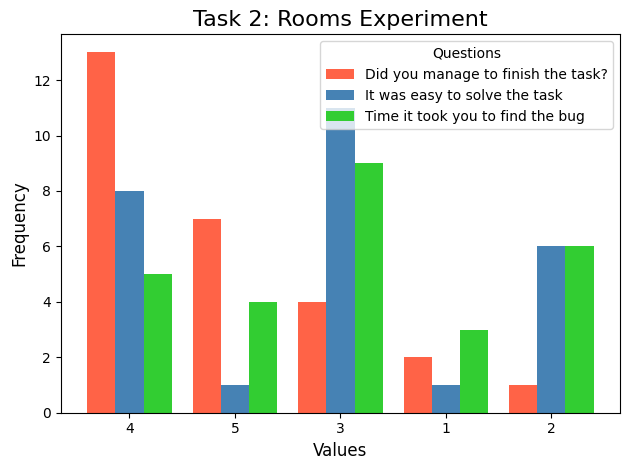
\includegraphics[width=0.5\textwidth]{figures/task2.png}
    \caption{Results Task 2}
    \label{fig:task2}
\end{figure}

cars

\begin{table}[!h]
\centering
\resizebox{\columnwidth}{!}{%
\begin{tabular}{
>{\columncolor[HTML]{FFFFFF}}c 
>{\columncolor[HTML]{FFFFFF}}c 
>{\columncolor[HTML]{FFFFFF}}c 
>{\columncolor[HTML]{FFFFFF}}c }
\multicolumn{4}{c}{\cellcolor[HTML]{FFFFFF}{\color[HTML]{000000} \textbf{Task 3: Cars Experiment.}}}                                                                                                                                           \\
{\color[HTML]{000000} \textbf{Values}} & {\color[HTML]{000000} \textbf{Did you manage to finish the task?}} & {\color[HTML]{000000} \textbf{It was easy to solve the task}} & {\color[HTML]{000000} \textbf{Time it took you to find the bug}} \\
{\color[HTML]{000000} \textbf{5}}      & {\color[HTML]{000000} 8}                                           & {\color[HTML]{000000} 2}                                      & {\color[HTML]{000000} 6}                                         \\
{\color[HTML]{000000} \textbf{3}}      & {\color[HTML]{000000} 6}                                           & {\color[HTML]{000000} 7}                                      & {\color[HTML]{000000} 6}                                         \\
{\color[HTML]{000000} \textbf{4}}      & {\color[HTML]{000000} 6}                                           & {\color[HTML]{000000} 4}                                      & {\color[HTML]{000000} 5}                                         \\
{\color[HTML]{000000} \textbf{2}}      & {\color[HTML]{000000} 4}                                           & {\color[HTML]{000000} 10}                                     & {\color[HTML]{000000} 7}                                         \\
{\color[HTML]{000000} \textbf{1}}      & {\color[HTML]{000000} 3}                                           & {\color[HTML]{000000} 4}                                      & {\color[HTML]{000000} 3}                                        
\end{tabular}%
}
\end{table}

\begin{figure}[h]
    \centering
    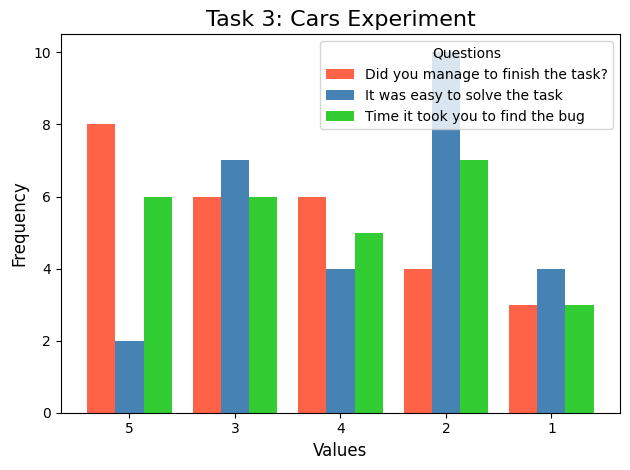
\includegraphics[width=0.5\textwidth]{figures/task3.png}
    \caption{Results Task 3}
    \label{fig:task3}
\end{figure}

\section{Debugger Usability Results}
\label{sec:usability}

\begin{table}[]
\centering
\resizebox{\columnwidth}{!}{%
\begin{tabular}{
>{\columncolor[HTML]{FFFFFF}}c 
>{\columncolor[HTML]{FFFFFF}}c 
>{\columncolor[HTML]{FFFFFF}}c 
>{\columncolor[HTML]{FFFFFF}}c 
>{\columncolor[HTML]{FFFFFF}}c 
>{\columncolor[HTML]{FFFFFF}}c 
>{\columncolor[HTML]{FFFFFF}}c 
>{\columncolor[HTML]{FFFFFF}}c 
>{\columncolor[HTML]{FFFFFF}}c 
>{\columncolor[HTML]{FFFFFF}}c 
>{\columncolor[HTML]{FFFFFF}}c }
\multicolumn{11}{c}{\cellcolor[HTML]{FFFFFF}{\color[HTML]{383838} \textbf{Debugger Usability.}}}                                                                                                                                                                                                                                                                                                                                                                                                                                                                                                                                                                                                                                                                                                                                                                                                                                                                                                                                                                                                                                                                                                                                                                                                                                                         \\
{\color[HTML]{383838} \textbf{}}  & {\color[HTML]{383838} \textbf{\begin{tabular}[c]{@{}c@{}}I think I would like to use this \\ system frequently\end{tabular}}} & {\color[HTML]{383838} \textbf{\begin{tabular}[c]{@{}c@{}}I find this system \\ unnecessarily complex\end{tabular}}} & {\color[HTML]{383838} \textbf{\begin{tabular}[c]{@{}c@{}}I think the system \\ is easy to use\end{tabular}}} & {\color[HTML]{383838} \textbf{\begin{tabular}[c]{@{}c@{}}I think I would need technical \\ support to use the system\end{tabular}}} & {\color[HTML]{383838} \textbf{\begin{tabular}[c]{@{}c@{}}I find the various functions of the \\ system quite well integrated\end{tabular}}} & {\color[HTML]{383838} \textbf{\begin{tabular}[c]{@{}c@{}}I have found too much \\ inconsistency in this system\end{tabular}}} & {\color[HTML]{383838} \textbf{\begin{tabular}[c]{@{}c@{}}I think most people would learn \\ to use the system quickly\end{tabular}}} & {\color[HTML]{383838} \textbf{\begin{tabular}[c]{@{}c@{}}I found the system quite \\ awkward to use\end{tabular}}} & {\color[HTML]{383838} \textbf{\begin{tabular}[c]{@{}c@{}}I have felt very safe \\ using the system\end{tabular}}} & {\color[HTML]{383838} \textbf{\begin{tabular}[c]{@{}c@{}}I would need to learn a lot \\ of things before I could handle the system\end{tabular}}} \\
{\color[HTML]{383838} \textbf{5}} & {\color[HTML]{383838} 7}                                                                                                      & {\color[HTML]{383838} 2}                                                                                            & {\color[HTML]{383838} 5.0}                                                                                   & {\color[HTML]{383838} 9}                                                                                                            & {\color[HTML]{383838} 6}                                                                                                                    & {\color[HTML]{383838} 1}                                                                                                      & {\color[HTML]{383838} 7}                                                                                                             & {\color[HTML]{383838} 4}                                                                                           & {\color[HTML]{383838} 7}                                                                                          & {\color[HTML]{383838} 8.0}                                                                                                                        \\
{\color[HTML]{383838} \textbf{2}} & {\color[HTML]{383838} 7}                                                                                                      & {\color[HTML]{383838} 6}                                                                                            & {\color[HTML]{383838} 6.0}                                                                                   & {\color[HTML]{383838} 3}                                                                                                            & {\color[HTML]{383838} 2}                                                                                                                    & {\color[HTML]{383838} 7}                                                                                                      & {\color[HTML]{383838} 6}                                                                                                             & {\color[HTML]{383838} 4}                                                                                           & {\color[HTML]{383838} 4}                                                                                          & {\color[HTML]{383838} NaN}                                                                                                                        \\
{\color[HTML]{383838} \textbf{3}} & {\color[HTML]{383838} 7}                                                                                                      & {\color[HTML]{383838} 7}                                                                                            & {\color[HTML]{383838} 11.0}                                                                                  & {\color[HTML]{383838} 4}                                                                                                            & {\color[HTML]{383838} 5}                                                                                                                    & {\color[HTML]{383838} 4}                                                                                                      & {\color[HTML]{383838} 6}                                                                                                             & {\color[HTML]{383838} 9}                                                                                           & {\color[HTML]{383838} 7}                                                                                          & {\color[HTML]{383838} 4.0}                                                                                                                        \\
{\color[HTML]{383838} \textbf{4}} & {\color[HTML]{383838} 5}                                                                                                      & {\color[HTML]{383838} 7}                                                                                            & {\color[HTML]{383838} 5.0}                                                                                   & {\color[HTML]{383838} 8}                                                                                                            & {\color[HTML]{383838} 13}                                                                                                                   & {\color[HTML]{383838} 2}                                                                                                      & {\color[HTML]{383838} 6}                                                                                                             & {\color[HTML]{383838} 7}                                                                                           & {\color[HTML]{383838} 8}                                                                                          & {\color[HTML]{383838} 6.0}                                                                                                                        \\
{\color[HTML]{383838} \textbf{1}} & {\color[HTML]{383838} 1}                                                                                                      & {\color[HTML]{383838} 5}                                                                                            & {\color[HTML]{383838} NaN}                                                                                   & {\color[HTML]{383838} 3}                                                                                                            & {\color[HTML]{383838} 1}                                                                                                                    & {\color[HTML]{383838} 13}                                                                                                     & {\color[HTML]{383838} 2}                                                                                                             & {\color[HTML]{383838} 3}                                                                                           & {\color[HTML]{383838} 1}                                                                                          & {\color[HTML]{383838} 9.0}                                                                                                                       
\end{tabular}%
}
\end{table}

\section{Discussion}
\label{sec:discussion}




\endinput

